% Options for packages loaded elsewhere
% Options for packages loaded elsewhere
\PassOptionsToPackage{unicode}{hyperref}
\PassOptionsToPackage{hyphens}{url}
%
\documentclass[
  ignorenonframetext,
]{beamer}
\newif\ifbibliography
\usepackage{pgfpages}
\setbeamertemplate{caption}[numbered]
\setbeamertemplate{caption label separator}{: }
\setbeamercolor{caption name}{fg=normal text.fg}
\beamertemplatenavigationsymbolsempty
% remove section numbering
\setbeamertemplate{part page}{
  \centering
  \begin{beamercolorbox}[sep=16pt,center]{part title}
    \usebeamerfont{part title}\insertpart\par
  \end{beamercolorbox}
}
\setbeamertemplate{section page}{
  \centering
  \begin{beamercolorbox}[sep=12pt,center]{section title}
    \usebeamerfont{section title}\insertsection\par
  \end{beamercolorbox}
}
\setbeamertemplate{subsection page}{
  \centering
  \begin{beamercolorbox}[sep=8pt,center]{subsection title}
    \usebeamerfont{subsection title}\insertsubsection\par
  \end{beamercolorbox}
}
% Prevent slide breaks in the middle of a paragraph
\widowpenalties 1 10000
\raggedbottom
\AtBeginPart{
  \frame{\partpage}
}
\AtBeginSection{
  \ifbibliography
  \else
    \frame{\sectionpage}
  \fi
}
\AtBeginSubsection{
  \frame{\subsectionpage}
}
\usepackage{iftex}
\ifPDFTeX
  \usepackage[T1]{fontenc}
  \usepackage[utf8]{inputenc}
  \usepackage{textcomp} % provide euro and other symbols
\else % if luatex or xetex
  \usepackage{unicode-math} % this also loads fontspec
  \defaultfontfeatures{Scale=MatchLowercase}
  \defaultfontfeatures[\rmfamily]{Ligatures=TeX,Scale=1}
\fi
\usepackage{lmodern}

\usetheme[]{default}
\ifPDFTeX\else
  % xetex/luatex font selection
\fi
% Use upquote if available, for straight quotes in verbatim environments
\IfFileExists{upquote.sty}{\usepackage{upquote}}{}
\IfFileExists{microtype.sty}{% use microtype if available
  \usepackage[]{microtype}
  \UseMicrotypeSet[protrusion]{basicmath} % disable protrusion for tt fonts
}{}
\makeatletter
\@ifundefined{KOMAClassName}{% if non-KOMA class
  \IfFileExists{parskip.sty}{%
    \usepackage{parskip}
  }{% else
    \setlength{\parindent}{0pt}
    \setlength{\parskip}{6pt plus 2pt minus 1pt}}
}{% if KOMA class
  \KOMAoptions{parskip=half}}
\makeatother

\usepackage{color}
\usepackage{fancyvrb}
\newcommand{\VerbBar}{|}
\newcommand{\VERB}{\Verb[commandchars=\\\{\}]}
\DefineVerbatimEnvironment{Highlighting}{Verbatim}{commandchars=\\\{\}}
% Add ',fontsize=\small' for more characters per line
\usepackage{framed}
\definecolor{shadecolor}{RGB}{241,243,245}
\newenvironment{Shaded}{\begin{snugshade}}{\end{snugshade}}
\newcommand{\AlertTok}[1]{\textcolor[rgb]{0.68,0.00,0.00}{#1}}
\newcommand{\AnnotationTok}[1]{\textcolor[rgb]{0.37,0.37,0.37}{#1}}
\newcommand{\AttributeTok}[1]{\textcolor[rgb]{0.40,0.45,0.13}{#1}}
\newcommand{\BaseNTok}[1]{\textcolor[rgb]{0.68,0.00,0.00}{#1}}
\newcommand{\BuiltInTok}[1]{\textcolor[rgb]{0.00,0.23,0.31}{#1}}
\newcommand{\CharTok}[1]{\textcolor[rgb]{0.13,0.47,0.30}{#1}}
\newcommand{\CommentTok}[1]{\textcolor[rgb]{0.37,0.37,0.37}{#1}}
\newcommand{\CommentVarTok}[1]{\textcolor[rgb]{0.37,0.37,0.37}{\textit{#1}}}
\newcommand{\ConstantTok}[1]{\textcolor[rgb]{0.56,0.35,0.01}{#1}}
\newcommand{\ControlFlowTok}[1]{\textcolor[rgb]{0.00,0.23,0.31}{\textbf{#1}}}
\newcommand{\DataTypeTok}[1]{\textcolor[rgb]{0.68,0.00,0.00}{#1}}
\newcommand{\DecValTok}[1]{\textcolor[rgb]{0.68,0.00,0.00}{#1}}
\newcommand{\DocumentationTok}[1]{\textcolor[rgb]{0.37,0.37,0.37}{\textit{#1}}}
\newcommand{\ErrorTok}[1]{\textcolor[rgb]{0.68,0.00,0.00}{#1}}
\newcommand{\ExtensionTok}[1]{\textcolor[rgb]{0.00,0.23,0.31}{#1}}
\newcommand{\FloatTok}[1]{\textcolor[rgb]{0.68,0.00,0.00}{#1}}
\newcommand{\FunctionTok}[1]{\textcolor[rgb]{0.28,0.35,0.67}{#1}}
\newcommand{\ImportTok}[1]{\textcolor[rgb]{0.00,0.46,0.62}{#1}}
\newcommand{\InformationTok}[1]{\textcolor[rgb]{0.37,0.37,0.37}{#1}}
\newcommand{\KeywordTok}[1]{\textcolor[rgb]{0.00,0.23,0.31}{\textbf{#1}}}
\newcommand{\NormalTok}[1]{\textcolor[rgb]{0.00,0.23,0.31}{#1}}
\newcommand{\OperatorTok}[1]{\textcolor[rgb]{0.37,0.37,0.37}{#1}}
\newcommand{\OtherTok}[1]{\textcolor[rgb]{0.00,0.23,0.31}{#1}}
\newcommand{\PreprocessorTok}[1]{\textcolor[rgb]{0.68,0.00,0.00}{#1}}
\newcommand{\RegionMarkerTok}[1]{\textcolor[rgb]{0.00,0.23,0.31}{#1}}
\newcommand{\SpecialCharTok}[1]{\textcolor[rgb]{0.37,0.37,0.37}{#1}}
\newcommand{\SpecialStringTok}[1]{\textcolor[rgb]{0.13,0.47,0.30}{#1}}
\newcommand{\StringTok}[1]{\textcolor[rgb]{0.13,0.47,0.30}{#1}}
\newcommand{\VariableTok}[1]{\textcolor[rgb]{0.07,0.07,0.07}{#1}}
\newcommand{\VerbatimStringTok}[1]{\textcolor[rgb]{0.13,0.47,0.30}{#1}}
\newcommand{\WarningTok}[1]{\textcolor[rgb]{0.37,0.37,0.37}{\textit{#1}}}

\usepackage{longtable,booktabs,array}
\usepackage{calc} % for calculating minipage widths
\usepackage{caption}
% Make caption package work with longtable
\makeatletter
\def\fnum@table{\tablename~\thetable}
\makeatother
\usepackage{graphicx}
\makeatletter
\newsavebox\pandoc@box
\newcommand*\pandocbounded[1]{% scales image to fit in text height/width
  \sbox\pandoc@box{#1}%
  \Gscale@div\@tempa{\textheight}{\dimexpr\ht\pandoc@box+\dp\pandoc@box\relax}%
  \Gscale@div\@tempb{\linewidth}{\wd\pandoc@box}%
  \ifdim\@tempb\p@<\@tempa\p@\let\@tempa\@tempb\fi% select the smaller of both
  \ifdim\@tempa\p@<\p@\scalebox{\@tempa}{\usebox\pandoc@box}%
  \else\usebox{\pandoc@box}%
  \fi%
}
% Set default figure placement to htbp
\def\fps@figure{htbp}
\makeatother

\ifLuaTeX
  \usepackage{luacolor}
  \usepackage[soul]{lua-ul}
\else
  \usepackage{soul}
  \makeatletter
  \let\HL\hl
  \renewcommand\hl{% fix for beamer highlighting
    \let\set@color\beamerorig@set@color
    \let\reset@color\beamerorig@reset@color
    \HL}
  \makeatother
\fi




\setlength{\emergencystretch}{3em} % prevent overfull lines

\providecommand{\tightlist}{%
  \setlength{\itemsep}{0pt}\setlength{\parskip}{0pt}}



 


\makeatletter
\@ifpackageloaded{tcolorbox}{}{\usepackage[skins,breakable]{tcolorbox}}
\@ifpackageloaded{fontawesome5}{}{\usepackage{fontawesome5}}
\definecolor{quarto-callout-color}{HTML}{909090}
\definecolor{quarto-callout-note-color}{HTML}{0758E5}
\definecolor{quarto-callout-important-color}{HTML}{CC1914}
\definecolor{quarto-callout-warning-color}{HTML}{EB9113}
\definecolor{quarto-callout-tip-color}{HTML}{00A047}
\definecolor{quarto-callout-caution-color}{HTML}{FC5300}
\definecolor{quarto-callout-color-frame}{HTML}{acacac}
\definecolor{quarto-callout-note-color-frame}{HTML}{4582ec}
\definecolor{quarto-callout-important-color-frame}{HTML}{d9534f}
\definecolor{quarto-callout-warning-color-frame}{HTML}{f0ad4e}
\definecolor{quarto-callout-tip-color-frame}{HTML}{02b875}
\definecolor{quarto-callout-caution-color-frame}{HTML}{fd7e14}
\makeatother
\makeatletter
\@ifpackageloaded{caption}{}{\usepackage{caption}}
\AtBeginDocument{%
\ifdefined\contentsname
  \renewcommand*\contentsname{Table of contents}
\else
  \newcommand\contentsname{Table of contents}
\fi
\ifdefined\listfigurename
  \renewcommand*\listfigurename{List of Figures}
\else
  \newcommand\listfigurename{List of Figures}
\fi
\ifdefined\listtablename
  \renewcommand*\listtablename{List of Tables}
\else
  \newcommand\listtablename{List of Tables}
\fi
\ifdefined\figurename
  \renewcommand*\figurename{Figure}
\else
  \newcommand\figurename{Figure}
\fi
\ifdefined\tablename
  \renewcommand*\tablename{Table}
\else
  \newcommand\tablename{Table}
\fi
}
\@ifpackageloaded{float}{}{\usepackage{float}}
\floatstyle{ruled}
\@ifundefined{c@chapter}{\newfloat{codelisting}{h}{lop}}{\newfloat{codelisting}{h}{lop}[chapter]}
\floatname{codelisting}{Listing}
\newcommand*\listoflistings{\listof{codelisting}{List of Listings}}
\makeatother
\makeatletter
\makeatother
\makeatletter
\@ifpackageloaded{caption}{}{\usepackage{caption}}
\@ifpackageloaded{subcaption}{}{\usepackage{subcaption}}
\makeatother

\usepackage{bookmark}
\IfFileExists{xurl.sty}{\usepackage{xurl}}{} % add URL line breaks if available
\urlstyle{same}
\hypersetup{
  pdftitle={Multinomial Regression},
  pdfauthor={Suyog Chandramouli},
  hidelinks,
  pdfcreator={LaTeX via pandoc}}


\title{Multinomial Regression}
\subtitle{Princeton University}
\author{Suyog Chandramouli}
\date{2026-03-02}

\begin{document}
\frame{\titlepage}


\begin{frame}[fragile]{Packages}
\phantomsection\label{packages}
\begin{Shaded}
\begin{Highlighting}[]
\FunctionTok{library}\NormalTok{(tidyverse)}
\FunctionTok{library}\NormalTok{(easystats)}
\FunctionTok{library}\NormalTok{(marginaleffects)}
\FunctionTok{library}\NormalTok{(effects)}
\FunctionTok{library}\NormalTok{(ordinal)}
\FunctionTok{library}\NormalTok{(nnet)}
\FunctionTok{library}\NormalTok{(ggeffects)}
\FunctionTok{library}\NormalTok{(emmeans)}
\FunctionTok{library}\NormalTok{(car)}
\FunctionTok{library}\NormalTok{(knitr)}
\FunctionTok{library}\NormalTok{(patchwork)}
\FunctionTok{library}\NormalTok{(MASS)}
\FunctionTok{library}\NormalTok{(broom)}
\FunctionTok{library}\NormalTok{(modelsummary)}

\FunctionTok{options}\NormalTok{(}\AttributeTok{scipen =} \DecValTok{999}\NormalTok{)}
\end{Highlighting}
\end{Shaded}

\begin{itemize}
\tightlist
\item
  Access the .qmd document here:
  \url{https://github.com/suyoghc/PSY504_Spring_2026/tree/main/posts}
\end{itemize}

\note{\begin{itemize}
\tightlist
\item
  \textbf{New package today --- nnet.}
\end{itemize}

\begin{itemize}
\tightlist
\item
  \textbf{It contains the main function that we will be using to build
  multinomial regression models! It ships with base R. Just load it.}
\end{itemize}

\begin{itemize}
\tightlist
\item
  \textbf{Nnet stands for neural nets!}
\end{itemize}

\begin{itemize}
\tightlist
\item
  \textbf{There is a connection between the 2: A single-layer neural net
  with softmax output is just multinomial logistic regression wearing a
  different hat!}
\end{itemize}}
\end{frame}

\begin{frame}[fragile]{Today}
\phantomsection\label{today}
\begin{columns}[T]
\begin{column}{0.5\linewidth}
\begin{itemize}
\item
  From ordinal to multinomial
\item
  A motivating simulation: Career roulette

  \begin{itemize}
  \tightlist
  \item
    Why ordinal regression breaks
  \item
    Category-specific slopes
  \item
    The softmax / baseline-category idea
  \end{itemize}
\end{itemize}
\end{column}

\begin{column}{0.5\linewidth}
\begin{itemize}
\item
  Application: NHANES health ratings

  \begin{itemize}
  \tightlist
  \item
    Model fitting with \texttt{nnet::multinom()}
  \item
    Parameter interpretation
  \item
    Model comparisons
  \item
    Visualizing predicted probabilities
  \item
    Reporting
  \end{itemize}
\end{itemize}
\end{column}
\end{columns}

\note{\begin{itemize}
\item
  \textbf{starting off similar to logistic regression, and ordinal
  regression,}
\item
  \textbf{with a simple example to build intuition about what's going on
  under the hood with multinomial regression.}
\item
  \textbf{Logistic: Binary outcomes (biased coin).}
\item
  \textbf{Ordinal: Loaded dice.}
\item
  \textbf{The career roulette simulation is our loaded dice equivalent.}
\item
  \textbf{Second half is the NHANES application.}
\end{itemize}}
\end{frame}

\begin{frame}{Last week: Ordinal regression}
\phantomsection\label{last-week-ordinal-regression}
\begin{itemize}
\item
  Ordered outcomes: Low \textless{} Medium \textless{} High
\item
  We modeled \textbf{cumulative probabilities} \(P(Y \leq k)\) using the
  logit link
\end{itemize}

\note{\begin{itemize}
\item
  \textbf{Two weeks ago --- binary logistic. Yes/no, pass/fail.}
\item
  \textbf{Last time we extended that to ordered categories. The key move
  was cumulative probabilities --- P of Y less than or equal to k.}
\end{itemize}}

\pause

\[\text{logit}\big(P(Y \leq k)\big) = \alpha_k - \beta X\]

\note{\emph{Quick recap. Two weeks ago --- binary logistic. Yes/no,
pass/fail. Last time we extended that to ordered categories. The key
move was cumulative probabilities --- P of Y less than or equal to k.}

\textbf{Alpha-k are thresholds, beta is the slope.}}

\pause

\begin{itemize}
\tightlist
\item
  We assumed one shared slope (β) --- the proportional odds
  assumption.\\
  (to keep things simple)
\end{itemize}

\note{\emph{Quick recap. Two weeks ago --- binary logistic. Yes/no,
pass/fail. Last time we extended that to ordered categories. The key
move was cumulative probabilities --- P of Y less than or equal to k.}

\emph{Here's the equation. Same one from last time. Alpha-k are
thresholds, beta is the slope.}

\textbf{constraint --- proportional odds.\\
\strut \\
One shared slope across all cumulative splits. K minus 1 thresholds but
only one beta. That's what made it parsimonious.}}

\pause

\begin{tcolorbox}[enhanced jigsaw, colbacktitle=quarto-callout-note-color!10!white, toptitle=1mm, colframe=quarto-callout-note-color-frame, toprule=.15mm, arc=.35mm, bottomtitle=1mm, opacityback=0, bottomrule=.15mm, left=2mm, title=\textcolor{quarto-callout-note-color}{\faInfo}\hspace{0.5em}{Note}, coltitle=black, leftrule=.75mm, rightrule=.15mm, titlerule=0mm, colback=white, opacitybacktitle=0.6, breakable]

Today: What happens when your outcome categories have \textbf{no natural
ordering}?

\end{tcolorbox}

\note{\textbf{Now we relax that entirely. What if the categories don't
have an order at all?}}
\end{frame}

\begin{frame}{Ordinal response variables (recap)}
\phantomsection\label{ordinal-response-variables-recap}
\begin{itemize}
\item
  Last time we saw outcomes with a clear ranking

  \begin{itemize}
  \tightlist
  \item
    Graduate school likelihood: unlikely \textless{} somewhat likely
    \textless{} very likely
  \item
    Loaded dice: Low \textless{} Medium \textless{} High
  \item
    Health status: poor \textless{} fair \textless{} good \textless{}
    excellent
  \end{itemize}
\end{itemize}

\note{\begin{itemize}
\tightlist
\item
  \textbf{These are all from last lecture and the lab. Grad school
  likelihood --- our real data application. Loaded dice --- our
  simulation. Health status --- your chapter reading. In every case,
  there's a clear ordering. ``Unlikely'' is less than ``somewhat
  likely'' is less than ``very likely.''}
\end{itemize}}

\pause

\begin{itemize}
\tightlist
\item
  Cumulative splits made sense because the categories \emph{stack}
\end{itemize}

\note{\emph{These are all from last lecture and the lab. Grad school
likelihood --- our real data application. Loaded dice --- our
simulation. Health status --- your chapter reading. In every case,
there's a clear ordering. ``Unlikely'' is less than ``somewhat likely''
is less than ``very likely.''}

\textbf{Cumulative splits respect that stacking --- P of Y less than or
equal to k. But what happens when you can't stack?}}
\end{frame}

\begin{frame}[fragile]{But not everything is ordered}
\phantomsection\label{but-not-everything-is-ordered}
\begin{columns}[T]
\begin{column}{0.5\linewidth}
\textbf{Ordered} (ordinal regression)

\begin{itemize}
\tightlist
\item
  Pain severity: mild \textless{} moderate \textless{} severe
\item
  Agreement: disagree \textless{} neutral \textless{} agree
\item
  Grades: C \textless{} B \textless{} A
\end{itemize}
\end{column}

\begin{column}{0.5\linewidth}
\textbf{Unordered} (??? regression)

\begin{itemize}
\tightlist
\item
  Political party: Democrat, Republican, Independent
\item
  Study strategy: space, light cram, heavy cram
\item
  Therapy type: CBT, DBT, psychodynamic
\end{itemize}
\end{column}
\end{columns}

\note{\begin{itemize}
\item
  \textbf{There's a direction, a ladder.}
\item
  \textbf{These are just\ldots{} different.}
\end{itemize}}

\pause

\begin{tcolorbox}[enhanced jigsaw, colbacktitle=quarto-callout-warning-color!10!white, toptitle=1mm, colframe=quarto-callout-warning-color-frame, toprule=.15mm, arc=.35mm, bottomtitle=1mm, opacityback=0, bottomrule=.15mm, left=2mm, title=\textcolor{quarto-callout-warning-color}{\faExclamationTriangle}\hspace{0.5em}{The problem}, coltitle=black, leftrule=.75mm, rightrule=.15mm, titlerule=0mm, colback=white, opacitybacktitle=0.6, breakable]

Can you say Democrat \textless{} Republican \textless{} Independent? Is
CBT \textless{} DBT \textless{} psychodynamic?

There's no meaningful way to rank these. Cumulative splits don't make
sense.

\end{tcolorbox}

\note{\begin{itemize}
\tightlist
\item
  \textbf{Can you say Democrat is less than Republican? Is CBT less than
  psychodynamic?}
\end{itemize}

\begin{itemize}
\tightlist
\item
  \textbf{If there's no ranking, you can't do cumulative splits.}
\end{itemize}

\begin{verbatim}
-   **P of Y less than or equal to Republican doesn't mean anything.**
\end{verbatim}
}
\end{frame}

\begin{frame}{Liu Ch 7 reading}
\phantomsection\label{liu-ch-7-reading}
Liu uses \textbf{health status} (poor, fair, good, excellent) as the
outcome.

\note{\textbf{Liu uses health status --- poor, fair, good, excellent ---
as the outcome in a multinomial model.}}

\pause

Isn't that ordinal?!

\note{\emph{So here's a fun tension from your reading. Liu uses health
status --- poor, fair, good, excellent --- as the outcome in a
multinomial model.}

\textbf{But wait. We literally just spent an entire lecture modeling
that kind of variable with ordinal regression. So why is Liu using
multinomial?}}

\pause

Liu explicitly acknowledges this:

\begin{quote}
\emph{``Although the multinomial logistic regression model is normally
used to estimate nominal response variables, it is an alternative to
estimate ordinal response variables when the proportional odds
assumption is violated.''}
\end{quote}

\note{\textbf{Multinomial is an alternative when proportional odds
doesn't hold.}}

\pause

\begin{tcolorbox}[enhanced jigsaw, colbacktitle=quarto-callout-note-color!10!white, toptitle=1mm, colframe=quarto-callout-note-color-frame, toprule=.15mm, arc=.35mm, bottomtitle=1mm, opacityback=0, bottomrule=.15mm, left=2mm, title=\textcolor{quarto-callout-note-color}{\faInfo}\hspace{0.5em}{Note}, coltitle=black, leftrule=.75mm, rightrule=.15mm, titlerule=0mm, colback=white, opacitybacktitle=0.6, breakable]

Two reasons to use multinomial regression:

\begin{enumerate}
\tightlist
\item
  The outcome is \textbf{genuinely unordered} (party affiliation,
  therapy choice)
\item
  The outcome is ordinal but \textbf{proportional odds fails} (fallback
  option)
\end{enumerate}

Today we focus on reason 1 --- the outcome truly has no order.

\end{tcolorbox}

\note{\textbf{But I want to be clear. That's reason two --- the
fallback. The stronger reason is reason one: the outcome is genuinely
unordered. That's where multinomial isn't just a fallback --- it's the
correct choice. That's our focus today.}

Remember: if proportional odds fails for only some predictors,
\textbf{partial proportional odds} is the first thing to try.
Multinomial is the nuclear option --- it drops \textbf{all} ordering
information.}
\end{frame}

\begin{frame}{What goes wrong if we force an order?}
\phantomsection\label{what-goes-wrong-if-we-force-an-order}
Imagine 3 career paths --- \textbf{academia}, \textbf{industry},
\textbf{government}, and 1 predictor, years of work experience.

\note{\textbf{Let's make this concrete. Three career paths --- academia,
industry, government. One predictor --- years of work experience.}}

\pause

\begin{itemize}
\item
  Experience pushes people \emph{toward} industry and \emph{away from}
  academia, but has little effect on government
\item
  There's no natural ordering: academia is not ``less than'' government
\end{itemize}

\note{\emph{Let's make this concrete. Three career paths --- academia,
industry, government. One predictor --- years of work experience.}

\textbf{Here's the truth we'll bake into the simulation: experience
pushes people toward industry and away from academia. Government stays
roughly flat. And there's no natural ordering --- academia isn't ``less
than'' government.}}

\pause

\textbf{If we force an ordering} (academia = 1, government = 2, industry
= 3) and fit an ordinal model:

\note{\emph{Let's make this concrete. Three career paths --- academia,
industry, government. One predictor --- years of work experience.}

\emph{Here's the truth we'll bake into the simulation: experience pushes
people toward industry and away from academia. Government stays roughly
flat. And there's no natural ordering --- academia isn't ``less than''
government.}

\textbf{But what if we forced one anyway? Code academia as 1, government
as 2, industry as 3. Run an ordinal model.}}

\pause

\begin{itemize}
\tightlist
\item
  The model assumes one shared slope --- but the true effect is
  \textbf{different for each category}
\item
  Proportional odds is violated by design
\item
  The single slope averages over contradictory effects
\end{itemize}

\note{\textbf{The ordinal model estimates one shared slope. But the true
effect is contradictory --- experience increases industry odds and
decreases academia odds. One slope averages them into mush. Proportional
odds is violated by design.}}

\pause

\begin{tcolorbox}[enhanced jigsaw, colbacktitle=quarto-callout-important-color!10!white, toptitle=1mm, colframe=quarto-callout-important-color-frame, toprule=.15mm, arc=.35mm, bottomtitle=1mm, opacityback=0, bottomrule=.15mm, left=2mm, title=\textcolor{quarto-callout-important-color}{\faExclamation}\hspace{0.5em}{The key difference}, coltitle=black, leftrule=.75mm, rightrule=.15mm, titlerule=0mm, colback=white, opacitybacktitle=0.6, breakable]

Ordinal regression: \textbf{K − 1 thresholds, 1 slope} per predictor
(shared across splits)

Multinomial regression: \textbf{K − 1 intercepts, K − 1 slopes} per
predictor (each category gets its own)

\end{tcolorbox}

\note{\emph{Let's make this concrete. Three career paths --- academia,
industry, government. One predictor --- years of work experience.}

\emph{Here's the truth we'll bake into the simulation: experience pushes
people toward industry and away from academia. Government stays roughly
flat. And there's no natural ordering --- academia isn't ``less than''
government.}

\emph{But what if we forced one anyway? Code academia as 1, government
as 2, industry as 3. Run an ordinal model.}

\emph{The ordinal model estimates one shared slope. But the true effect
is contradictory --- experience increases industry odds and decreases
academia odds. One slope averages them into mush. Proportional odds is
violated by design.}

\textbf{And that's the key difference. Ordinal: K minus 1 thresholds,
one slope. Multinomial: K minus 1 intercepts, K minus 1 slopes. Each
category gets its own. That extra flexibility is exactly what you need
when effects go in different directions.}}
\end{frame}

\begin{frame}{The connection across models}
\phantomsection\label{the-connection-across-models}
\[\begin{array}{lll}
\textbf{Logistic} & \text{2 categories} & \text{1 intercept, 1 slope} \\[6pt]
\textbf{Ordinal} & \text{K ordered categories} & \text{K−1 thresholds, } \mathbf{1} \text{ slope (shared)} \\[6pt]
\textbf{Multinomial} & \text{K unordered categories} & \text{K−1 intercepts, } \mathbf{K−1} \text{ slopes (category-specific)}
\end{array}\]

\note{\textbf{Here's the whole arc in one slide. Logistic --- two
categories, one intercept, one slope. That was week one. Ordinal --- K
ordered categories, K minus 1 thresholds, but still just one slope.
That's the proportional odds constraint. And now multinomial --- K
unordered categories, K minus 1 intercepts, K minus 1 slopes.}}

\pause

\begin{columns}[T]
\begin{column}{0.5\linewidth}
\textbf{Ordinal} (last time)

\[\begin{aligned}
L_1 &= \alpha_1 - \beta x \\
L_2 &= \alpha_2 - \beta x \\
L_{K-1} &= \alpha_{K-1} - \beta x
\end{aligned}\]

Same \(\beta\) everywhere --- proportional odds
\end{column}

\begin{column}{0.5\linewidth}
\textbf{Multinomial} (today)

\[\begin{aligned}
L_1 &= \alpha_1 + \beta_1 x \\
L_2 &= \alpha_2 + \beta_2 x \\
L_{K-1} &= \alpha_{K-1} + \beta_{K-1} x
\end{aligned}\]

Each category gets its \textbf{own} \(\beta_j\)
\end{column}
\end{columns}

\note{\emph{Here's the whole arc in one slide. Logistic --- two
categories, one intercept, one slope. That was week one. Ordinal --- K
ordered categories, K minus 1 thresholds, but still just one slope.
That's the proportional odds constraint. And now multinomial --- K
unordered categories, K minus 1 intercepts, K minus 1 slopes.}

\textbf{Look at the equations side by side. On the left, ordinal ---
same beta everywhere. On the right, multinomial --- beta-1, beta-2,
beta-K-minus-1. Every category gets its own relationship with the
predictor. That's the one structural change. Everything else --- the
logit link, maximum likelihood, the log-odds interpretation --- stays
the same. We're just relaxing the shared-slope constraint.}}
\end{frame}

\begin{frame}[fragile]{Multinomial logistic regression}
\phantomsection\label{multinomial-logistic-regression}
\begin{itemize}
\tightlist
\item
  Choose a \textbf{baseline category} (reference). All comparisons are
  relative to it.
\end{itemize}

\note{\textbf{Here's the formal setup. Pick one category as the baseline
--- the reference. Every other category gets compared to it.}}

\pause

\begin{itemize}
\tightlist
\item
  If the outcome has \(K\) categories and the baseline is category
  \(K\), we model \(K - 1\) log-odds:
\end{itemize}

\[\log\bigg(\frac{P(Y = j)}{P(Y = K)}\bigg) = \beta_{0j} + \beta_{1j} x_1 + \cdots + \beta_{pj} x_p\]

for \(j = 1, 2, \ldots, K-1\)

\note{\emph{Here's the formal setup. Pick one category as the baseline
--- the reference. Every other category gets compared to it.}

\textbf{If you have K categories, you write K minus 1 log-odds
equations. Each one looks like a logistic regression. But notice the
subscript j on every beta --- each equation has its own coefficients.}

\textbf{category-specific log-odds relative to a baseline}}

\pause

\begin{itemize}
\item
  Each equation is its own logistic regression --- but they're estimated
  \textbf{simultaneously}
\item
  The chapter calls these \texttt{log(mu{[},2{]}/mu{[},1{]})},
  \texttt{log(mu{[},3{]}/mu{[},1{]})}, etc.
\end{itemize}

\note{\emph{Here's the formal setup. Pick one category as the baseline
--- the reference. Every other category gets compared to it.}

\emph{If you have K categories, you write K minus 1 log-odds equations.
Each one looks like a logistic regression. But notice the subscript j on
every beta --- each equation has its own coefficients.}

\textbf{They're estimated simultaneously, not independently. The model
sees all the data at once. The chapter notation --- log of mu 2 over mu
1, log of mu 3 over mu 1 --- that's exactly this. Mu 1 is the
baseline.}}

\pause

\begin{tcolorbox}[enhanced jigsaw, colbacktitle=quarto-callout-tip-color!10!white, toptitle=1mm, colframe=quarto-callout-tip-color-frame, toprule=.15mm, arc=.35mm, bottomtitle=1mm, opacityback=0, bottomrule=.15mm, left=2mm, title=\textcolor{quarto-callout-tip-color}{\faLightbulb}\hspace{0.5em}{Interpretation}, coltitle=black, leftrule=.75mm, rightrule=.15mm, titlerule=0mm, colback=white, opacitybacktitle=0.6, breakable]

\(\beta_{1j}\): when \(x_1\) increases by one unit, the log-odds of
being in category \(j\) \textbf{vs.~the baseline} change by
\(\beta_{1j}\)

\(\exp(\beta_{1j})\): the \textbf{odds ratio} --- the multiplicative
change in odds of category \(j\) vs.~baseline

\end{tcolorbox}

\note{\emph{Here's the formal setup. Pick one category as the baseline
--- the reference. Every other category gets compared to it.}

\emph{If you have K categories, you write K minus 1 log-odds equations.
Each one looks like a logistic regression. But notice the subscript j on
every beta --- each equation has its own coefficients.}

\emph{They're estimated simultaneously, not independently. The model
sees all the data at once. The chapter notation --- log of mu 2 over mu
1, log of mu 3 over mu 1 --- that's exactly this. Mu 1 is the baseline.}

\textbf{Interpretation. Beta-1-j is the change in log-odds of category j
versus baseline when x goes up by one. Exponentiate and you get the odds
ratio. Same as logistic regression, just specific to one comparison.}}
\end{frame}

\begin{frame}{Multinomial distribution}
\phantomsection\label{multinomial-distribution}
\begin{itemize}
\item
  Extension of Bernoulli and binomial distributions
\item
  When you have more than two outcomes and fixed number of trials
\end{itemize}

\[P(X_1 = x_1, X_2 = x_2, \ldots, X_k = x_k) = \frac{n!}{x_1! x_2! \cdots x_k!} p_1^{x_1} p_2^{x_2} \cdots p_k^{x_k}\]

\begin{itemize}
\tightlist
\item
  \(X\) = \# of times events occur
\item
  \(p\) = probability of occurrence
\item
  \(n\) = \# of trials
\end{itemize}

\[\text{Mean of } X_i = E[X_i] = n \cdot p_i\]\[\text{Variance of } X_i = \text{Var}(X_i) = n \cdot p_i \cdot (1 - p_i)\]
\end{frame}

\begin{frame}{Multinomial Logistic Regression}
\phantomsection\label{multinomial-logistic-regression-1}
\begin{itemize}
\tightlist
\item
  In ordinal regression:
\end{itemize}

\[\begin{array}{rcl} L_1 &=& \alpha_1-\beta_1x_1-\cdots-\beta_p X_p\\ L_2 &=& \alpha_2-\beta_1x_1-\cdots-\beta_p X_p & \\ L_{J-1} &=& \alpha_{J-1}-\beta_1x_1-\cdots-\beta_p X_p \end{array}\]

\begin{itemize}
\tightlist
\item
  In the multinomial logistic model:
\end{itemize}

\[\begin{array}{rcl} L_1 &=& \alpha_1+\beta_1x_1+\cdots+\beta_p X_p\\ L_2 &=& \alpha_2+\beta_2x_1+\cdots+\beta_p X_p & \\ L_{J-1} &=& \alpha_{J-1}+\beta_jx_1+\cdots+\beta_p X_p \end{array}\]
\end{frame}

\begin{frame}{Multinomial logistic regression}
\phantomsection\label{multinomial-logistic-regression-2}
\begin{itemize}
\tightlist
\item
  Choose a baseline category. Let's choose \(y=0\). Then,
\end{itemize}

\[P(y_i = 0|x_i) = P_{i0}\] and \[P(y_i = 1|x_i) = P_{i1}\]

\[\log\bigg(\frac{p_{i1}}{p_{i0}}\bigg) = \beta_{0k} + \beta_{1k} x_i\]

\begin{itemize}
\item
  Slope: \(\beta_1\): when x increases by one unit, the odds of Y = 1
  vs.~baseline is expected to multiply by a factor or \(exp(\beta)\)
\item
  Intercept: \(\beta_0\): when x = 0 the odds of Y = 1 is expected to be
  \(exp(\beta)\)
\end{itemize}
\end{frame}

\begin{frame}{Think of it as simultaneous binary regressions}
\phantomsection\label{think-of-it-as-simultaneous-binary-regressions}
\pandocbounded{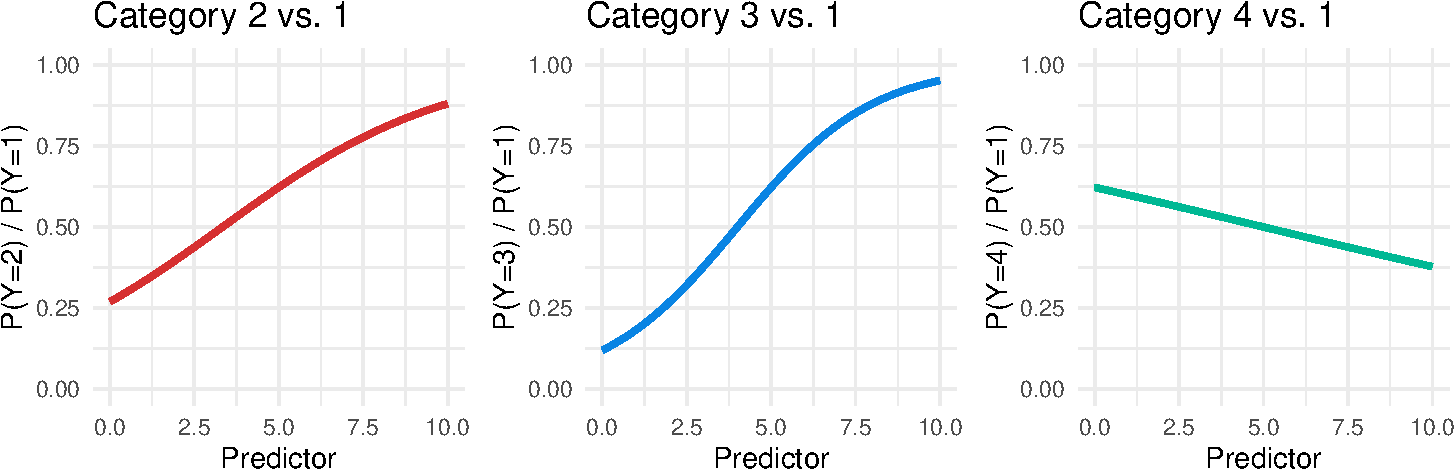
\includegraphics[keepaspectratio]{multinomial_regression_lecture1_files/figure-beamer/unnamed-chunk-2-1.pdf}}

\note{\textbf{Three panels, three comparisons --- all versus baseline
category 1. Look at the slopes. Red --- category 2 vs.~1, positive
slope, predictor pushes odds up. Blue --- category 3 vs.~1, even
steeper. Green --- category 4 vs.~1, slightly negative. Predictor pushes
you away from this one.}}

\pause

Each comparison has its \textbf{own intercept and slope}. The predictor
can push \emph{toward} one category and \emph{away from} another ---
something ordinal regression cannot do.

\note{\emph{Three panels, three comparisons --- all versus baseline
category 1. Look at the slopes. Red --- category 2 vs.~1, positive
slope, predictor pushes odds up. Blue --- category 3 vs.~1, even
steeper. Green --- category 4 vs.~1, slightly negative. Predictor pushes
you away from this one.}

\textbf{This is what ordinal regression cannot do. One slope can't go up
for some categories and down for others. Here, each comparison is free
to go its own direction. That's the whole point of multinomial.}}
\end{frame}

\section{Under the Hood: Career
Roulette}\label{under-the-hood-career-roulette}

\begin{frame}{The career roulette}
\phantomsection\label{the-career-roulette}
Easier to understand multinomial regression if we \textbf{simulate it
from scratch} and watch each step.

\note{\textbf{That's the conceptual setup. You know why multinomial
exists --- unordered categories need category-specific slopes. You know
the equation --- K minus 1 log-odds comparisons to a baseline.}}

\pause

Just like our loaded dice helped us understand ordinal regression.

\note{\emph{That's the conceptual setup. You know why multinomial exists
--- unordered categories need category-specific slopes. You know the
equation --- K minus 1 log-odds comparisons to a baseline.}

\textbf{Now let's build it from scratch. Same philosophy as the loaded
dice --- set true parameters, generate data, see if the model recovers
what we planted. Except instead of dice landing on Low, Medium, High ---
we have people choosing careers.}}
\end{frame}

\begin{frame}[fragile]{The DGP: Career paths}
\phantomsection\label{the-dgp-career-paths}
300 people choosing among \textbf{3 careers} based on years of work
experience.

\begin{Shaded}
\begin{Highlighting}[]
\FunctionTok{set.seed}\NormalTok{(}\DecValTok{504}\NormalTok{)}

\NormalTok{n }\OtherTok{\textless{}{-}} \DecValTok{300}
\NormalTok{experience }\OtherTok{\textless{}{-}} \FunctionTok{runif}\NormalTok{(n, }\DecValTok{0}\NormalTok{, }\DecValTok{20}\NormalTok{)}

\CommentTok{\# ── TRUE PARAMETERS (log{-}odds vs. Government baseline) ──}
\NormalTok{b0\_acad }\OtherTok{\textless{}{-}} \FloatTok{1.0}\NormalTok{;  b1\_acad }\OtherTok{\textless{}{-}} \SpecialCharTok{{-}}\FloatTok{0.15}   \CommentTok{\# academia: popular early, fades}
\NormalTok{b0\_ind  }\OtherTok{\textless{}{-}} \SpecialCharTok{{-}}\FloatTok{0.5}\NormalTok{; b1\_ind  }\OtherTok{\textless{}{-}}  \FloatTok{0.20}   \CommentTok{\# industry: unpopular early, rises}

\CommentTok{\# Linear predictors (Government is reference. Fixed at 0)}
\NormalTok{score\_govt }\OtherTok{\textless{}{-}} \FunctionTok{rep}\NormalTok{(}\DecValTok{0}\NormalTok{, n)}
\NormalTok{score\_acad }\OtherTok{\textless{}{-}}\NormalTok{ b0\_acad }\SpecialCharTok{+}\NormalTok{ b1\_acad }\SpecialCharTok{*}\NormalTok{ experience}
\NormalTok{score\_ind  }\OtherTok{\textless{}{-}}\NormalTok{ b0\_ind  }\SpecialCharTok{+}\NormalTok{ b1\_ind  }\SpecialCharTok{*}\NormalTok{ experience}
\end{Highlighting}
\end{Shaded}

\note{\textbf{Here's our data generating process.}

\begin{itemize}
\item
  SELECT

  \begin{itemize}
  \tightlist
  \item
    \textbf{Three hundred people, each with some years of work
    experience drawn uniformly from 0 to 20.}
  \end{itemize}
\item
  \textbf{They choose one of three careers --- academia, industry, or
  government.}

  \begin{itemize}
  \item
    \textbf{The key: government is our reference category, so its score
    is fixed at zero.}

    \begin{itemize}
    \tightlist
    \item
      \textbf{Academia and industry each get their own intercept and
      their own slope.}
    \end{itemize}
  \end{itemize}
\end{itemize}}

\pause

\begin{tcolorbox}[enhanced jigsaw, colbacktitle=quarto-callout-note-color!10!white, toptitle=1mm, colframe=quarto-callout-note-color-frame, toprule=.15mm, arc=.35mm, bottomtitle=1mm, opacityback=0, bottomrule=.15mm, left=2mm, title=\textcolor{quarto-callout-note-color}{\faInfo}\hspace{0.5em}{The truth we're planting}, coltitle=black, leftrule=.75mm, rightrule=.15mm, titlerule=0mm, colback=white, opacitybacktitle=0.6, breakable]

\begin{itemize}
\tightlist
\item
  \textbf{Academia vs.~Government}: intercept = 1.0, slope =
  \textbf{−0.15} (experience pulls \emph{away})

  \begin{itemize}
  \tightlist
  \item
    The \textbf{intercept} says: \emph{at 0 years of experience, how
    attractive is this category relative to Government?}

    \begin{itemize}
    \tightlist
    \item
      The \textbf{slope} says: \emph{as experience increases, does this
      category become more or less attractive relative to Government?}
    \end{itemize}
  \end{itemize}
\item
  \textbf{Industry vs.~Government}: intercept = −0.5, slope =
  \textbf{+0.20} (experience pushes \emph{toward})
\item
  \textbf{Government}: baseline (score = 0 by definition)
\end{itemize}

\end{tcolorbox}

\note{\textbf{Look at the slopes ---}

\begin{itemize}
\item
  \textbf{they go in opposite directions.}

  \begin{itemize}
  \item
    \textbf{More experience pushes you away from academia and toward
    industry.}
  \item
    We are literally setting different slopes and generating data

    \begin{itemize}
    \item
      \textbf{That's why ordinal regression can't work here.}
    \item
      \textbf{One slope can't be both negative and positive.}
    \end{itemize}
  \end{itemize}
\end{itemize}}
\end{frame}

\begin{frame}{Softmax in action}
\phantomsection\label{softmax-in-action}
How do linear predictors become probabilities? Take one person with
\textbf{experience = 5 years}:

\note{\textbf{Before we generate the full dataset, let's see what
actually happens here?}

``here is the formula for softmax

``here is how the model becomes a stochastic data-generating process''

\begin{itemize}
\item
  We've done something like thist wice already

  \begin{itemize}
  \item
    in logistic regression, we took a (1) log-odds score into a
    probability. plogis

    \begin{itemize}
    \item
      That was softmax with two categories.
    \item
      you applied plogis to each threshold to get cumulative
      probabilities, then subtracted to get category probabilities.
    \end{itemize}
  \item
    \textbf{Now we have three categories} competing for probability

    \begin{itemize}
    \item
      so the denominator gets bigger.
    \item
      It's the same idea, now with more players.\textbf{\hfill\break
      }
    \end{itemize}
  \end{itemize}
\end{itemize}

\begin{itemize}
\item
  \textbf{1) How does the model turn linear predictors into
  probabilities?}

  \begin{itemize}
  \tightlist
  \item
    \textbf{Let's pick one person with five years of experience and
    trace every step.}
  \end{itemize}
\end{itemize}}

\pause

\textbf{Step 1}: Compute scores

\[\text{score}_{\text{acad}} = 1.0 + (-0.15)(5) = 0.25 \qquad \text{score}_{\text{ind}} = -0.5 + (0.20)(5) = 0.50 \qquad \text{score}_{\text{govt}} = 0\]

\note{\begin{itemize}
\item
  \textbf{Step one}

  \begin{itemize}
  \item
    \textbf{plug experience into the linear predictors.}

    \begin{itemize}
    \item
      \textbf{Academia gets 0.25, industry gets 0.50, government is zero
      by definition.}
    \item
      \ul{\textbf{These are log-odds-scale scores}}\textbf{.}

      \begin{itemize}
      \tightlist
      \item
        \textbf{Not probabilities yet.}
      \end{itemize}
    \end{itemize}
  \end{itemize}
\item
  \begin{quote}
  ``These scores are the category-specific log-odds relative to
  Government; softmax turns them into probabilities.''
  \end{quote}
\end{itemize}}

\pause

\textbf{Step 2}: Exponentiate → \textbf{Step 3}: Normalize (divide by
sum)

\[p_k = \frac{\exp(\text{score}_k)}{\sum_j \exp(\text{score}_j)} \quad \Rightarrow \quad p_{\text{acad}} = \frac{e^{0.25}}{e^{0.25} + e^{0.50} + e^{0}} = \frac{1.28}{3.93} = 0.33\]

\[p_{\text{ind}} = \frac{1.65}{3.93} = 0.42 \qquad p_{\text{govt}} = \frac{1.00}{3.93} = 0.25\]

\note{\emph{How does the model turn linear predictors into
probabilities? Let's pick one person with five years of experience and
trace every step.}

\emph{Step one --- plug experience into the linear predictors.}

\textbf{Step two --- exponentiate each score.}

\textbf{Step three --- divide by the sum.}

\begin{itemize}
\item
  \textbf{That's softmax.}

  \begin{itemize}
  \tightlist
  \item
    \textbf{For this person, industry has a 42 percent chance, academia
    33, government 25. The highest score wins the most probability, but
    nobody gets zero --- everyone has some chance.}
  \end{itemize}
\end{itemize}}

\pause

\textbf{Step 4}: Sample one career with those probabilities → this
person happens to choose \textbf{Industry}

\note{\emph{How does the model turn linear predictors into
probabilities? Let's pick one person with five years of experience and
trace every step.}

\emph{Step one --- plug experience into the linear predictors.}

\begin{itemize}
\tightlist
\item
  \emph{Academia gets 0.25, industry gets 0.50, government is zero by
  definition. These are log-odds-scale scores. Not probabilities yet.}
\end{itemize}

\emph{Step two --- exponentiate each score. That's softmax.}

\begin{itemize}
\tightlist
\item
  \emph{For this person, industry has a 42 percent chance, academia 33,
  government 25. The highest score wins the most probability, but nobody
  gets zero --- everyone has some chance.}
\end{itemize}

\textbf{Step four}

\begin{itemize}
\item
  \textbf{we sample one career from those probabilities.}

  \begin{itemize}
  \tightlist
  \item
    \textbf{This person lands on industry. Now repeat 300 times, and you
    have a dataset.}
  \end{itemize}
\end{itemize}}
\end{frame}

\begin{frame}[fragile]{Generating the data}
\phantomsection\label{generating-the-data}
\begin{Shaded}
\begin{Highlighting}[]
\CommentTok{\# Softmax → probabilities}
\NormalTok{denom  }\OtherTok{\textless{}{-}} \FunctionTok{exp}\NormalTok{(score\_govt) }\SpecialCharTok{+} \FunctionTok{exp}\NormalTok{(score\_acad) }\SpecialCharTok{+} \FunctionTok{exp}\NormalTok{(score\_ind)}
\NormalTok{p\_govt }\OtherTok{\textless{}{-}} \FunctionTok{exp}\NormalTok{(score\_govt) }\SpecialCharTok{/}\NormalTok{ denom}
\NormalTok{p\_acad }\OtherTok{\textless{}{-}} \FunctionTok{exp}\NormalTok{(score\_acad) }\SpecialCharTok{/}\NormalTok{ denom}
\NormalTok{p\_ind  }\OtherTok{\textless{}{-}} \FunctionTok{exp}\NormalTok{(score\_ind)  }\SpecialCharTok{/}\NormalTok{ denom}

\CommentTok{\# Sample one career per person}
\NormalTok{career }\OtherTok{\textless{}{-}} \FunctionTok{sapply}\NormalTok{(}\DecValTok{1}\SpecialCharTok{:}\NormalTok{n, }\ControlFlowTok{function}\NormalTok{(i) \{}
  \FunctionTok{sample}\NormalTok{(}\FunctionTok{c}\NormalTok{(}\StringTok{"Academia"}\NormalTok{, }\StringTok{"Industry"}\NormalTok{, }\StringTok{"Government"}\NormalTok{),}
         \AttributeTok{size =} \DecValTok{1}\NormalTok{,}
         \AttributeTok{prob =} \FunctionTok{c}\NormalTok{(p\_acad[i], p\_ind[i], p\_govt[i]))}
\NormalTok{\})}

\NormalTok{sim\_data }\OtherTok{\textless{}{-}} \FunctionTok{tibble}\NormalTok{(}
  \AttributeTok{experience =}\NormalTok{ experience,}
  \AttributeTok{career     =} \FunctionTok{factor}\NormalTok{(career, }\AttributeTok{levels =} \FunctionTok{c}\NormalTok{(}\StringTok{"Government"}\NormalTok{, }\StringTok{"Academia"}\NormalTok{, }\StringTok{"Industry"}\NormalTok{))}
\NormalTok{)}

\NormalTok{sim\_data }\SpecialCharTok{\%\textgreater{}\%} \FunctionTok{count}\NormalTok{(career)}
\end{Highlighting}
\end{Shaded}

\begin{verbatim}
# A tibble: 3 x 2
  career         n
  <fct>      <int>
1 Government    48
2 Academia      52
3 Industry     200
\end{verbatim}

\note{\textbf{Here's the code doing exactly what we just traced out}

\begin{itemize}
\item
  \textbf{softmax probabilities for all 300 people,}

  \begin{itemize}
  \item
    \textbf{then one random career draw each.}

    \begin{itemize}
    \tightlist
    \item
      \textbf{Notice we set Government as the first factor level}
    \end{itemize}

\begin{verbatim}
-   **— that makes it the baseline when we fit the model later.**
\end{verbatim}
  \end{itemize}
\end{itemize}}
\end{frame}

\begin{frame}{\textbf{The underlying data-generating process}}
\phantomsection\label{the-underlying-data-generating-process}
\pandocbounded{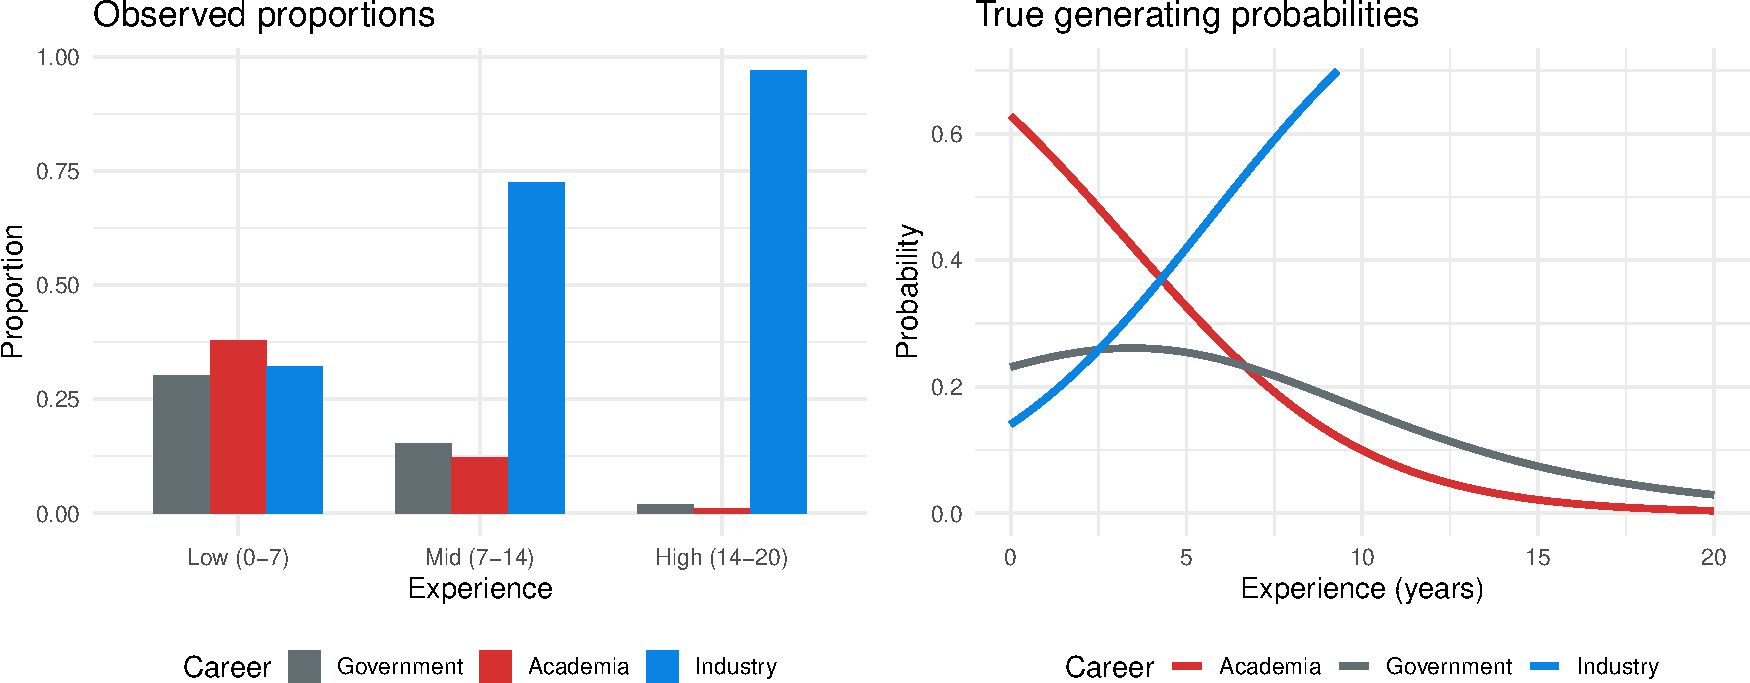
\includegraphics[keepaspectratio]{multinomial_regression_lecture1_files/figure-beamer/unnamed-chunk-5-1.pdf}}

\note{\textbf{Two panels.}

\begin{itemize}
\item
  \textbf{Left --- the observed data,}

  \begin{itemize}
  \tightlist
  \item
    \textbf{binned into low, medium, and high experience.}
  \end{itemize}
\item
  \textbf{Watch the pattern:}

  \begin{itemize}
  \item
    \textbf{academia dominates at low experience,}

    \begin{itemize}
    \tightlist
    \item
      \textbf{industry rises, government stays middling.}
    \end{itemize}
  \end{itemize}
\item
  \textbf{Right --- the true probability curves we baked in.}

  \begin{itemize}
  \tightlist
  \item
    \textbf{The data on the left is a noisy snapshot of the smooth
    curves on the right.}
  \end{itemize}
\end{itemize}

\textbf{Even though we are dealing with a linear model in the linear
predictor scale.} Because in multinomial regression, what is linear are
the \textbf{category-specific log-odds relative to the reference
category}.}

\pause

The careers \textbf{trade places} as experience increases. No single
gradient can capture this.

\note{\textbf{This is the key visual.}

\begin{itemize}
\tightlist
\item
  \textbf{The careers trade places. At zero experience, academia leads.
  By twenty years, industry dominates. Government stays roughly flat.
  There is no single direction here --- no gradient from less to more.
  That's why this is genuinely unordered.}
\end{itemize}}
\end{frame}

\begin{frame}[fragile]{Exploring the simulated data}
\phantomsection\label{exploring-the-simulated-data}
\begin{Shaded}
\begin{Highlighting}[]
\CommentTok{\# Proportions at each experience bin}
\NormalTok{sim\_binned }\SpecialCharTok{\%\textgreater{}\%}
  \FunctionTok{count}\NormalTok{(exp\_bin, career) }\SpecialCharTok{\%\textgreater{}\%}
  \FunctionTok{group\_by}\NormalTok{(exp\_bin) }\SpecialCharTok{\%\textgreater{}\%}
  \FunctionTok{mutate}\NormalTok{(}
    \AttributeTok{prop =}\NormalTok{ n }\SpecialCharTok{/} \FunctionTok{sum}\NormalTok{(n),}
    \AttributeTok{log\_odds\_vs\_govt =} \FunctionTok{round}\NormalTok{(}\FunctionTok{log}\NormalTok{(prop }\SpecialCharTok{/}\NormalTok{ prop[career }\SpecialCharTok{==} \StringTok{"Government"}\NormalTok{]), }\DecValTok{3}\NormalTok{)}
\NormalTok{  ) }\SpecialCharTok{\%\textgreater{}\%}
  \FunctionTok{kable}\NormalTok{(}\AttributeTok{digits =} \DecValTok{3}\NormalTok{)}
\end{Highlighting}
\end{Shaded}

\begin{longtable}[]{@{}llrrr@{}}
\toprule\noalign{}
exp\_bin & career & n & prop & log\_odds\_vs\_govt \\
\midrule\noalign{}
\endhead
Low (0-7) & Government & 31 & 0.301 & 0.000 \\
Low (0-7) & Academia & 39 & 0.379 & 0.230 \\
Low (0-7) & Industry & 33 & 0.320 & 0.063 \\
Mid (7--14) & Government & 15 & 0.153 & 0.000 \\
Mid (7--14) & Academia & 12 & 0.122 & -0.223 \\
Mid (7--14) & Industry & 71 & 0.724 & 1.555 \\
High (14--20) & Government & 2 & 0.020 & 0.000 \\
High (14--20) & Academia & 1 & 0.010 & -0.693 \\
High (14--20) & Industry & 96 & 0.970 & 3.871 \\
\bottomrule\noalign{}
\end{longtable}

\note{\textbf{We computed the proportion choosing each career at low,
medium, and high experience.}

\begin{itemize}
\item
  \textbf{Then we take the log of each proportion \ul{divided by the
  government proportion}.}

  \begin{itemize}
  \tightlist
  \item
    \textbf{That gives us \ul{log-odds versus baseline at each
    experience level.}}
  \end{itemize}
\end{itemize}}

\pause

\begin{tcolorbox}[enhanced jigsaw, colbacktitle=quarto-callout-note-color!10!white, toptitle=1mm, colframe=quarto-callout-note-color-frame, toprule=.15mm, arc=.35mm, bottomtitle=1mm, opacityback=0, bottomrule=.15mm, left=2mm, title=\textcolor{quarto-callout-note-color}{\faInfo}\hspace{0.5em}{What do you notice?}, coltitle=black, leftrule=.75mm, rightrule=.15mm, titlerule=0mm, colback=white, opacitybacktitle=0.6, breakable]

The \textbf{log-odds of academia vs.~government} decrease as experience
goes up. The \textbf{log-odds of industry vs.~government} increase. Each
career has its own trend --- and the trends go in opposite directions.

\end{tcolorbox}

\note{\emph{Let's explore the data before modeling it. We compute the
proportion choosing each career at low, medium, and high experience.
Then we take the log of each proportion divided by the government
proportion. That gives us log-odds versus baseline at each experience
level.}

\textbf{Look at the pattern. Academia's log-odds drop as experience goes
up. Industry's log-odds rise. Two separate trends, opposite directions.
This is exactly what the model needs to capture --- and exactly what a
single shared slope cannot.}}
\end{frame}

\begin{frame}[fragile]{What if we force an order?}
\phantomsection\label{what-if-we-force-an-order}
Code the careers as \textbf{1 = Academia, 2 = Government, 3 = Industry}
and fit an ordinal model.

\begin{Shaded}
\begin{Highlighting}[]
\NormalTok{sim\_data\_ord }\OtherTok{\textless{}{-}}\NormalTok{ sim\_data }\SpecialCharTok{\%\textgreater{}\%}
  \FunctionTok{mutate}\NormalTok{(}\AttributeTok{career\_ord =} \FunctionTok{ordered}\NormalTok{(career, }
                              \AttributeTok{levels =} \FunctionTok{c}\NormalTok{(}\StringTok{"Academia"}\NormalTok{, }\StringTok{"Government"}\NormalTok{, }\StringTok{"Industry"}\NormalTok{)))}

\NormalTok{wrong\_model }\OtherTok{\textless{}{-}} \FunctionTok{clm}\NormalTok{(career\_ord }\SpecialCharTok{\textasciitilde{}}\NormalTok{ experience, }\AttributeTok{data =}\NormalTok{ sim\_data\_ord)}

\FunctionTok{tidy}\NormalTok{(wrong\_model) }\SpecialCharTok{\%\textgreater{}\%} \FunctionTok{kable}\NormalTok{(}\AttributeTok{digits =} \DecValTok{3}\NormalTok{)}
\end{Highlighting}
\end{Shaded}

\begin{longtable}[]{@{}
  >{\raggedright\arraybackslash}p{(\linewidth - 10\tabcolsep) * \real{0.3472}}
  >{\raggedleft\arraybackslash}p{(\linewidth - 10\tabcolsep) * \real{0.1250}}
  >{\raggedleft\arraybackslash}p{(\linewidth - 10\tabcolsep) * \real{0.1389}}
  >{\raggedleft\arraybackslash}p{(\linewidth - 10\tabcolsep) * \real{0.1389}}
  >{\raggedleft\arraybackslash}p{(\linewidth - 10\tabcolsep) * \real{0.1111}}
  >{\raggedright\arraybackslash}p{(\linewidth - 10\tabcolsep) * \real{0.1389}}@{}}
\toprule\noalign{}
\begin{minipage}[b]{\linewidth}\raggedright
term
\end{minipage} & \begin{minipage}[b]{\linewidth}\raggedleft
estimate
\end{minipage} & \begin{minipage}[b]{\linewidth}\raggedleft
std.error
\end{minipage} & \begin{minipage}[b]{\linewidth}\raggedleft
statistic
\end{minipage} & \begin{minipage}[b]{\linewidth}\raggedleft
p.value
\end{minipage} & \begin{minipage}[b]{\linewidth}\raggedright
coef.type
\end{minipage} \\
\midrule\noalign{}
\endhead
Academia\textbar Government & 0.583 & 0.252 & 2.312 & 0.021 &
intercept \\
Government\textbar Industry & 1.861 & 0.277 & 6.727 & 0.000 &
intercept \\
experience & 0.291 & 0.031 & 9.283 & 0.000 & location \\
\bottomrule\noalign{}
\end{longtable}

\note{\textbf{Now let's do what you should never do --- force an order.
We code academia as 1, government as 2, industry as 3 and fit a
cumulative logit model. The ordinal model estimates one shared slope for
experience. Let's see what it gives us.}}

\pause

\begin{Shaded}
\begin{Highlighting}[]
\CommentTok{\# Check proportional odds}
\FunctionTok{library}\NormalTok{(sure)}
\FunctionTok{set.seed}\NormalTok{(}\DecValTok{504}\NormalTok{)}
\FunctionTok{nominal\_test}\NormalTok{(wrong\_model)}
\end{Highlighting}
\end{Shaded}

\begin{verbatim}
Tests of nominal effects

formula: career_ord ~ experience
           Df  logLik    AIC     LRT Pr(>Chi)
<none>        -193.38 392.75                 
experience  1 -192.95 393.90 0.85183    0.356
\end{verbatim}

\note{\emph{Now let's do what you should never do --- force an order. We
code academia as 1, government as 2, industry as 3 and fit a cumulative
logit model. The ordinal model estimates one shared slope for
experience. Let's see what it gives us.}

\begin{itemize}
\item
  \textbf{And the nominal test rejects proportional odds. The assumption
  fails because the true effects go in opposite directions.}
\item
  \textbf{The shared slope is trying to average a negative effect and a
  positive effect into one number.}
\end{itemize}}
\end{frame}

\begin{frame}{Three things went wrong}
\phantomsection\label{three-things-went-wrong}
\begin{tcolorbox}[enhanced jigsaw, colbacktitle=quarto-callout-warning-color!10!white, toptitle=1mm, colframe=quarto-callout-warning-color-frame, toprule=.15mm, arc=.35mm, bottomtitle=1mm, opacityback=0, bottomrule=.15mm, left=2mm, title=\textcolor{quarto-callout-warning-color}{\faExclamationTriangle}\hspace{0.5em}{Why the ordinal model fails here}, coltitle=black, leftrule=.75mm, rightrule=.15mm, titlerule=0mm, colback=white, opacitybacktitle=0.6, breakable]

\begin{enumerate}
\item
  \textbf{No natural gradient exists} --- academia, government, and
  industry don't fall on a continuum. Any ordering we impose is
  arbitrary.
\item
  \textbf{One slope can't be both positive and negative} --- experience
  pushes \emph{toward} industry and \emph{away from} academia. A shared
  slope averages contradictory effects into mush.
\item
  \textbf{Proportional odds is violated by construction} --- the model
  assumes the same effect across cumulative splits, but the true
  category-specific effects differ in sign.
\end{enumerate}

\end{tcolorbox}

\note{\textbf{Three things went wrong, and they're all related. First
--- there's no real ordering. We picked academia less-than government
less-than industry, but that's arbitrary. Second --- the one-slope
constraint is fatal. Experience is positive for industry and negative
for academia. Average those and you get near zero --- the model misses
both effects. Third --- proportional odds is violated because the true
effects genuinely differ across categories. This isn't a borderline
assumption violation. It's fundamental.}}

\pause

We need a model that gives \textbf{each category its own slope}.

\note{\textbf{So we need a model with separate slopes --- one for each
comparison. That's exactly what multinomial gives us.}}
\end{frame}

\begin{frame}[fragile]{Multinomial model recovers the truth}
\phantomsection\label{multinomial-model-recovers-the-truth}
\begin{Shaded}
\begin{Highlighting}[]
\FunctionTok{library}\NormalTok{(nnet)}
\NormalTok{right\_model }\OtherTok{\textless{}{-}} \FunctionTok{multinom}\NormalTok{(career }\SpecialCharTok{\textasciitilde{}}\NormalTok{ experience, }\AttributeTok{data =}\NormalTok{ sim\_data, }\AttributeTok{trace =} \ConstantTok{FALSE}\NormalTok{)}

\FunctionTok{tidy}\NormalTok{(right\_model, }\AttributeTok{conf.int =} \ConstantTok{TRUE}\NormalTok{) }\SpecialCharTok{\%\textgreater{}\%}
  \FunctionTok{kable}\NormalTok{(}\AttributeTok{digits =} \DecValTok{3}\NormalTok{)}
\end{Highlighting}
\end{Shaded}

\begin{longtable}[]{@{}
  >{\raggedright\arraybackslash}p{(\linewidth - 14\tabcolsep) * \real{0.1169}}
  >{\raggedright\arraybackslash}p{(\linewidth - 14\tabcolsep) * \real{0.1558}}
  >{\raggedleft\arraybackslash}p{(\linewidth - 14\tabcolsep) * \real{0.1169}}
  >{\raggedleft\arraybackslash}p{(\linewidth - 14\tabcolsep) * \real{0.1299}}
  >{\raggedleft\arraybackslash}p{(\linewidth - 14\tabcolsep) * \real{0.1299}}
  >{\raggedleft\arraybackslash}p{(\linewidth - 14\tabcolsep) * \real{0.1039}}
  >{\raggedleft\arraybackslash}p{(\linewidth - 14\tabcolsep) * \real{0.1169}}
  >{\raggedleft\arraybackslash}p{(\linewidth - 14\tabcolsep) * \real{0.1299}}@{}}
\toprule\noalign{}
\begin{minipage}[b]{\linewidth}\raggedright
y.level
\end{minipage} & \begin{minipage}[b]{\linewidth}\raggedright
term
\end{minipage} & \begin{minipage}[b]{\linewidth}\raggedleft
estimate
\end{minipage} & \begin{minipage}[b]{\linewidth}\raggedleft
std.error
\end{minipage} & \begin{minipage}[b]{\linewidth}\raggedleft
statistic
\end{minipage} & \begin{minipage}[b]{\linewidth}\raggedleft
p.value
\end{minipage} & \begin{minipage}[b]{\linewidth}\raggedleft
conf.low
\end{minipage} & \begin{minipage}[b]{\linewidth}\raggedleft
conf.high
\end{minipage} \\
\midrule\noalign{}
\endhead
Academia & (Intercept) & 0.502 & 0.324 & 1.549 & 0.121 & -0.133 &
1.136 \\
Academia & experience & -0.082 & 0.050 & -1.654 & 0.098 & -0.180 &
0.015 \\
Industry & (Intercept) & -1.085 & 0.351 & -3.086 & 0.002 & -1.774 &
-0.396 \\
Industry & experience & 0.271 & 0.040 & 6.795 & 0.000 & 0.193 & 0.349 \\
\bottomrule\noalign{}
\end{longtable}

\note{\textbf{Now we fit the right model. multinom from the nnet
package. Government is our reference level. The model estimates two
intercepts and two slopes --- one for academia versus government, one
for industry versus government.}}

\pause

\begin{longtable}[]{@{}llrr@{}}
\toprule\noalign{}
Comparison & Term & True & Estimated \\
\midrule\noalign{}
\endhead
Academia vs.~Govt & (Intercept) & 1.00 & 0.502 \\
Academia vs.~Govt & experience & -0.15 & -0.082 \\
Industry vs.~Govt & (Intercept) & -0.50 & -1.085 \\
Industry vs.~Govt & experience & 0.20 & 0.271 \\
\bottomrule\noalign{}
\end{longtable}

\note{\emph{Now we fit the right model. multinom from the nnet package.
Government is our reference level. The model estimates two intercepts
and two slopes --- one for academia versus government, one for industry
versus government.}

\textbf{And here's the payoff --- true values next to estimated values.
The model recovers what we planted. The academia slope is negative, the
industry slope is positive, and the magnitudes are close to the truth.
The whole point of the simulation: fit the right model, get the right
answer.}}
\end{frame}

\begin{frame}[fragile]{Changing the baseline}
\phantomsection\label{changing-the-baseline}
What happens if we switch the reference from Government to Academia?

\begin{Shaded}
\begin{Highlighting}[]
\NormalTok{sim\_data\_reref }\OtherTok{\textless{}{-}}\NormalTok{ sim\_data }\SpecialCharTok{\%\textgreater{}\%}
  \FunctionTok{mutate}\NormalTok{(}\AttributeTok{career =} \FunctionTok{relevel}\NormalTok{(career, }\AttributeTok{ref =} \StringTok{"Academia"}\NormalTok{))}

\NormalTok{reref\_model }\OtherTok{\textless{}{-}} \FunctionTok{multinom}\NormalTok{(career }\SpecialCharTok{\textasciitilde{}}\NormalTok{ experience, }\AttributeTok{data =}\NormalTok{ sim\_data\_reref, }\AttributeTok{trace =} \ConstantTok{FALSE}\NormalTok{)}

\FunctionTok{tidy}\NormalTok{(reref\_model) }\SpecialCharTok{\%\textgreater{}\%} \FunctionTok{kable}\NormalTok{(}\AttributeTok{digits =} \DecValTok{3}\NormalTok{)}
\end{Highlighting}
\end{Shaded}

\begin{longtable}[]{@{}llrrrr@{}}
\toprule\noalign{}
y.level & term & estimate & std.error & statistic & p.value \\
\midrule\noalign{}
\endhead
Government & (Intercept) & -0.502 & 0.324 & -1.549 & 0.121 \\
Government & experience & 0.082 & 0.050 & 1.654 & 0.098 \\
Industry & (Intercept) & -1.586 & 0.354 & -4.486 & 0.000 \\
Industry & experience & 0.353 & 0.047 & 7.529 & 0.000 \\
\bottomrule\noalign{}
\end{longtable}

\note{\textbf{Common source of confusion --- what happens when you
change the baseline? Let's switch from government to academia as the
reference and refit. - The coefficients change. - Signs flip, magnitudes
shift. - But watch what happens to the predictions.}}

\pause

\begin{Shaded}
\begin{Highlighting}[]
\CommentTok{\# Predicted probabilities are identical}
\FunctionTok{bind\_rows}\NormalTok{(}
  \FunctionTok{predict}\NormalTok{(right\_model, }\AttributeTok{newdata =} \FunctionTok{tibble}\NormalTok{(}\AttributeTok{experience =} \DecValTok{10}\NormalTok{), }\AttributeTok{type =} \StringTok{"probs"}\NormalTok{) }\SpecialCharTok{\%\textgreater{}\%} 
    \FunctionTok{as\_tibble}\NormalTok{() }\SpecialCharTok{\%\textgreater{}\%} \FunctionTok{mutate}\NormalTok{(}\AttributeTok{baseline =} \StringTok{"Government"}\NormalTok{),}
  \FunctionTok{predict}\NormalTok{(reref\_model, }\AttributeTok{newdata =} \FunctionTok{tibble}\NormalTok{(}\AttributeTok{experience =} \DecValTok{10}\NormalTok{), }\AttributeTok{type =} \StringTok{"probs"}\NormalTok{) }\SpecialCharTok{\%\textgreater{}\%} 
    \FunctionTok{as\_tibble}\NormalTok{() }\SpecialCharTok{\%\textgreater{}\%} \FunctionTok{mutate}\NormalTok{(}\AttributeTok{baseline =} \StringTok{"Academia"}\NormalTok{)}
\NormalTok{) }\SpecialCharTok{\%\textgreater{}\%} \FunctionTok{kable}\NormalTok{(}\AttributeTok{digits =} \DecValTok{3}\NormalTok{)}
\end{Highlighting}
\end{Shaded}

\begin{longtable}[]{@{}rl@{}}
\toprule\noalign{}
value & baseline \\
\midrule\noalign{}
\endhead
0.147 & Government \\
0.107 & Government \\
0.746 & Government \\
0.107 & Academia \\
0.147 & Academia \\
0.746 & Academia \\
\bottomrule\noalign{}
\end{longtable}

\note{\emph{Common source of confusion --- what happens when you change
the baseline? Let's switch from government to academia as the reference
and refit. The coefficients change. Signs flip, magnitudes shift. But
watch what happens to the predictions.}

\textbf{Identical predicted probabilities. The model is the same ---
you're just reading a different column of the same table. Changing the
baseline changes how you describe the model, not what the model says.
Like converting temperatures from Fahrenheit to Celsius --- different
numbers, same weather.}}
\end{frame}

\begin{frame}[fragile]{Visualizing the recovery}
\phantomsection\label{visualizing-the-recovery}
\begin{Shaded}
\begin{Highlighting}[]
\CommentTok{\# True curves (from DGP) + fitted curves (from model)}
\NormalTok{fitted\_grid }\OtherTok{\textless{}{-}} \FunctionTok{tibble}\NormalTok{(}\AttributeTok{experience =} \FunctionTok{seq}\NormalTok{(}\DecValTok{0}\NormalTok{, }\DecValTok{20}\NormalTok{, }\FloatTok{0.1}\NormalTok{))}
\NormalTok{fitted\_probs }\OtherTok{\textless{}{-}} \FunctionTok{predict}\NormalTok{(right\_model, }\AttributeTok{newdata =}\NormalTok{ fitted\_grid, }\AttributeTok{type =} \StringTok{"probs"}\NormalTok{) }\SpecialCharTok{\%\textgreater{}\%}
  \FunctionTok{as\_tibble}\NormalTok{() }\SpecialCharTok{\%\textgreater{}\%}
  \FunctionTok{bind\_cols}\NormalTok{(fitted\_grid) }\SpecialCharTok{\%\textgreater{}\%}
  \FunctionTok{pivot\_longer}\NormalTok{(}\AttributeTok{cols =} \FunctionTok{c}\NormalTok{(Government, Academia, Industry),}
               \AttributeTok{names\_to =} \StringTok{"career"}\NormalTok{, }\AttributeTok{values\_to =} \StringTok{"fitted"}\NormalTok{)}

\NormalTok{true\_grid }\OtherTok{\textless{}{-}}\NormalTok{ exp\_grid }\SpecialCharTok{\%\textgreater{}\%} \FunctionTok{rename}\NormalTok{(}\AttributeTok{true\_prob =}\NormalTok{ prob)}

\NormalTok{combined }\OtherTok{\textless{}{-}}\NormalTok{ fitted\_probs }\SpecialCharTok{\%\textgreater{}\%}
  \FunctionTok{left\_join}\NormalTok{(true\_grid, }\AttributeTok{by =} \FunctionTok{c}\NormalTok{(}\StringTok{"experience"}\NormalTok{, }\StringTok{"career"}\NormalTok{))}

\FunctionTok{ggplot}\NormalTok{(combined, }\FunctionTok{aes}\NormalTok{(}\AttributeTok{x =}\NormalTok{ experience)) }\SpecialCharTok{+}
  \FunctionTok{geom\_line}\NormalTok{(}\FunctionTok{aes}\NormalTok{(}\AttributeTok{y =}\NormalTok{ true\_prob, }\AttributeTok{color =}\NormalTok{ career), }
            \AttributeTok{linetype =} \StringTok{"dashed"}\NormalTok{, }\AttributeTok{linewidth =} \FloatTok{1.2}\NormalTok{, }\AttributeTok{alpha =} \FloatTok{0.6}\NormalTok{) }\SpecialCharTok{+}
  \FunctionTok{geom\_line}\NormalTok{(}\FunctionTok{aes}\NormalTok{(}\AttributeTok{y =}\NormalTok{ fitted, }\AttributeTok{color =}\NormalTok{ career), }\AttributeTok{linewidth =} \FloatTok{1.2}\NormalTok{) }\SpecialCharTok{+}
  \FunctionTok{scale\_color\_manual}\NormalTok{(}\AttributeTok{values =} \FunctionTok{c}\NormalTok{(}\StringTok{"Government"} \OtherTok{=} \StringTok{"\#636e72"}\NormalTok{, }
                                 \StringTok{"Academia"}   \OtherTok{=} \StringTok{"\#d63031"}\NormalTok{, }
                                 \StringTok{"Industry"}   \OtherTok{=} \StringTok{"\#0984e3"}\NormalTok{)) }\SpecialCharTok{+}
  \FunctionTok{labs}\NormalTok{(}\AttributeTok{x =} \StringTok{"Experience (years)"}\NormalTok{, }\AttributeTok{y =} \StringTok{"Probability"}\NormalTok{,}
       \AttributeTok{title =} \StringTok{"Dashed = truth we planted | Solid = what the model found"}\NormalTok{,}
       \AttributeTok{color =} \StringTok{"Career"}\NormalTok{) }\SpecialCharTok{+}
  \FunctionTok{theme\_minimal}\NormalTok{(}\AttributeTok{base\_size =} \DecValTok{14}\NormalTok{) }\SpecialCharTok{+}
  \FunctionTok{theme}\NormalTok{(}\AttributeTok{legend.position =} \StringTok{"bottom"}\NormalTok{)}
\end{Highlighting}
\end{Shaded}

\pandocbounded{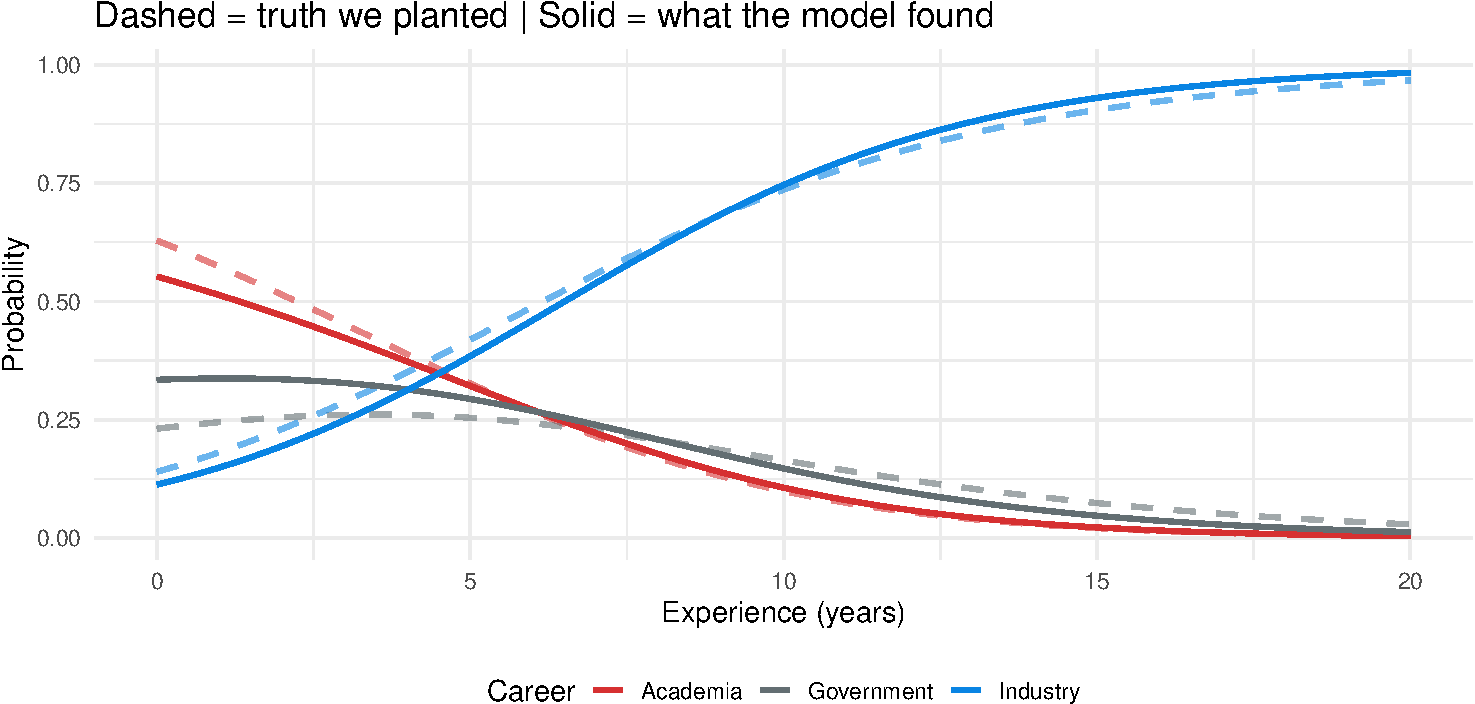
\includegraphics[keepaspectratio]{multinomial_regression_lecture1_files/figure-beamer/unnamed-chunk-13-1.pdf}}

\note{\textbf{Dashed lines are the truth we planted. Solid lines are
what the model estimated. They overlap. The model found the generating
process. This is the visual proof that multinomial regression works ---
it recovers category-specific effects that go in different directions.}}
\end{frame}

\begin{frame}[fragile]{Career roulette: Recap}
\phantomsection\label{career-roulette-recap}
\begin{longtable}[]{@{}
  >{\raggedright\arraybackslash}p{(\linewidth - 4\tabcolsep) * \real{0.2639}}
  >{\raggedright\arraybackslash}p{(\linewidth - 4\tabcolsep) * \real{0.3194}}
  >{\raggedright\arraybackslash}p{(\linewidth - 4\tabcolsep) * \real{0.4167}}@{}}
\toprule\noalign{}
\begin{minipage}[b]{\linewidth}\raggedright
Step
\end{minipage} & \begin{minipage}[b]{\linewidth}\raggedright
What we did
\end{minipage} & \begin{minipage}[b]{\linewidth}\raggedright
What it demonstrates
\end{minipage} \\
\midrule\noalign{}
\endhead
Define true parameters & Category-specific intercepts + slopes & Each
career gets its own relationship with experience \\
Softmax → sample & \texttt{exp(score)\ /\ sum(exp(scores))} & How linear
predictors become choice probabilities \\
Explore proportions & Log-odds vs.~baseline at each experience level &
Structure in the data mirrors what the model estimates \\
Fit ordinal model (wrong) & \texttt{clm()} gives one shared slope &
Proportional odds fails when effects differ by category \\
Fit multinomial model & \texttt{multinom()} recovers the truth &
Category-specific slopes capture contradictory effects \\
Change baseline & \texttt{relevel()} + refit & Coefficients change,
predictions don't \\
\bottomrule\noalign{}
\end{longtable}

\note{\textbf{Here's the full arc. We set the truth, generated data,
explored it, fit the wrong model, watched it fail, fit the right model,
and recovered what we planted. Same philosophy as the loaded dice ---
except now each category has its own slope instead of sharing one.}}

\pause

\begin{tcolorbox}[enhanced jigsaw, colbacktitle=quarto-callout-note-color!10!white, toptitle=1mm, colframe=quarto-callout-note-color-frame, toprule=.15mm, arc=.35mm, bottomtitle=1mm, opacityback=0, bottomrule=.15mm, left=2mm, title=\textcolor{quarto-callout-note-color}{\faInfo}\hspace{0.5em}{Note}, coltitle=black, leftrule=.75mm, rightrule=.15mm, titlerule=0mm, colback=white, opacitybacktitle=0.6, breakable]

Now let's apply this to real data --- where we don't know the truth.

\end{tcolorbox}

\note{\emph{Here's the full arc. We set the truth, generated data,
explored it, fit the wrong model, watched it fail, fit the right model,
and recovered what we planted. Same philosophy as the loaded dice ---
except now each category has its own slope instead of sharing one.}

\textbf{The chapter jumps straight to real data. We just did the step
Liu skips --- checking that the model works on data where we know the
answer. Now let's see what happens when we don't know the answer.}}
\end{frame}

\begin{frame}{Tomorrow - Stats Seminar}
\phantomsection\label{tomorrow---stats-seminar}
\pandocbounded{
\includegraphics[keepaspectratio]{images/clipboard-965951265.png}}

\note{Psychometrics: designing and evaluating tests that measure
psychological traits or abilities. Item Response Theory: models how a
person's latent trait affects their responses to individual test items.}
\end{frame}




\end{document}
